%%%%%%%%%%%%%%%%%%%%%%%%%%%%% Define Article %%%%%%%%%%%%%%%%%%%%%%%%%%%%%%%%%%
\documentclass{article}
%%%%%%%%%%%%%%%%%%%%%%%%%%%%%%%%%%%%%%%%%%%%%%%%%%%%%%%%%%%%%%%%%%%%%%%%%%%%%%%

%%%%%%%%%%%%%%%%%%%%%%%%%%%%% Using Packages %%%%%%%%%%%%%%%%%%%%%%%%%%%%%%%%%%
\usepackage{listings, xcolor}
\usepackage{parskip}
\usepackage{hyperref}
\usepackage{amsmath}
\usepackage{graphicx}
\usepackage[a4paper, margin = 1.5cm]{geometry}
\usepackage{float}
\usepackage{amssymb}

%%%%%%%%%%%%%%%%%%%%%%%%%%%%%%% Title & Author %%%%%%%%%%%%%%%%%%%%%%%%%%%%%%%%
\title{Diagramma delle Classi - Costruzione}
\author{Trentin Tommaso}
%%%%%%%%%%%%%%%%%%%%%%%%%%%%%%%%%%%%%%%%%%%%%%%%%%%%%%%%%%%%%%%%%%%%%%%%%%%%%%%

\begin{document}
  \maketitle
  \tableofcontents
  \newpage
  
  \section{Livelli di dettaglio}
    Diagrammi UML possono essere creati in diverse fasi del ciclo di vita, con diversi scopi / livelli di dettaglio:
    \begin{itemize}
      \item \textbf{System domain model}: modella entità del dominio del problema che saranno presenti nel sistema (dati di interesse), può contenere le responsabilità delle classi (opzionale); 
      \item \textbf{System model}: include anche classi che saranno usate per costruire il sistema completo (classi per interfaccia utente, classi associate a parti di architettura, classi di utility), oltre a metodi e informazioni sulla navigabilità. 
    \end{itemize}
  \section{Astrazione del System Domain Model}
    \begin{enumerate}
      \item Identificare primo insieme di \textbf{classi} candidate; 
      \item Aggiungere \textbf{associazioni} ed \textbf{attributi} delle classi;
      \item Trovare \textbf{generalizzazioni};
      \item Trovare principali \textbf{responsabilità} di ogni classe;
      \item Iterare processo finché modello ottenuto è soddisfacente.
    \end{enumerate}
    \subsection{Identificare Classi}
      Classi dovrebbero corrispondere a entità del dominio del problema, si applicano i concetti di OO: una classe identifica un tipo di dato astratto. Una buona classe:
      \begin{itemize}
        \item ha un nome che ne rispecchia l'intento; 
        \item è un'astrazione che modella un elemento del dominio del problema;
        \item ha insieme ridotto e ben definito di responsabilità.
      \end{itemize}
      \subsubsection{Analisi dei nomi}
        Semplice tecnica per scoprire le classi del dominio:
        \begin{enumerate}
          \item Analizzare documentazione di partenza; 
          \item Elencare i nomi; 
          \item Eliminare nomi che:
            \begin{itemize}
              \item sono ridondanti; 
              \item rappresentano / caratterizzano istanze e non classi;
              \item sono vaghi / generici;
              \item corrispondono a classi non necessarie al livello considerato.
            \end{itemize}
        \end{enumerate}
    \subsection{Identificare Attributi}
      \begin{itemize}
        \item Cercare informazioni da conservare per ciascuna classe; 
        \item Possibile che nomi scartati come classi al passo 1 ora possano essere considerati attributi;
        \item Una classe non dovrebbe avere troppi attributi;
        \item Bisogna stare attenti agli attributi contenenti molteplici valori.
      \end{itemize}
    \subsection{Identificare Associazioni}
      \begin{itemize}
        \item Espressioni verbali che coinvolgono più classi indicano possibili relazioni tra esse;
        \item Vanno cercate nell'ordine:
          \begin{enumerate}
            \item \textbf{Gen-Spec}: espressioni del tipo "è un";
            \item \textbf{Contenimento}: espressioni del tipo "è fatto di", "comprende";
            \item \textbf{Associazione}: ogni altra espressione.
          \end{enumerate} 
        \item Una volta identificata un'associazione:
          \begin{itemize}
            \item specificare molteplicità da entrambi i lati; 
            \item assegnare nome chiaro all'associazione e / o definire ruoli delle entità che partecipano all'associazione;
          \end{itemize}
      \end{itemize}
    \subsection{Identificare Generalizzazioni e Interfacce}
      Due modi principali per trovare \textbf{generalizzazioni}:
      \begin{itemize}
        \item Bottom-Up - ragruppando classi simili creando una nuova super-classe;
        \item Top-Down - creando prima classi più generali e poi specializzando.
      \end{itemize}
      Si crea invece un'\textbf{interfaccia} se: 
      \begin{itemize}
        \item classi sono molto diverse fra loro, tranne per alcune operazioni in comune; 
        \item potrebbero essere disponibili diverse implementazioni della stessa classe.
      \end{itemize}
    \subsection{Identificare Responsabilità}
      \begin{itemize}
        \item \textbf{Responsabilità} corrisponde a una funzionalità richiesta al sistema SW; 
        \item Responsabilità di ogni requisito funzionale va attribuita ad una delle classi, anche se nella pratica potrà essere svolto mediante collaborazione fra più classi; 
        \item Se classe ha troppe responsabilità, valutare di dividerla in più classi;
        \item Se classe non ha responsabilità, probabilmente è inutile;
        \item Se una responsabilità non può essere attribuita ad alcuna delle classi esistenti, probabilmente ne va creata una nuova; 
        \item Responsabilità di creare istanze di una classe non può essere attribuita alla classe stessa, ma ad una classe ad essa collegata (stessa cosa per collections tipo lista, catalogo... di); 
      \end{itemize}
      \begin{figure}[h!]
        \begin{center}
          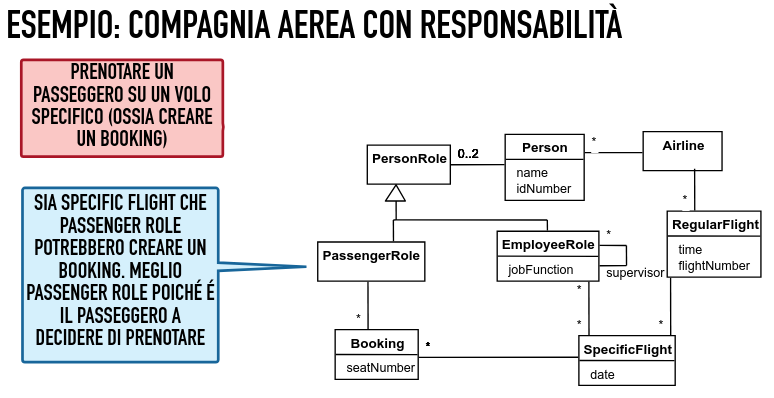
\includegraphics[width=0.5\textwidth]{figures/resp_es.png}
        \end{center}
      \end{figure}
      \subsubsection{Class Responsibility Collaboration (CRC) Cards}
        Metodo alternativo per ottenere diagramma delle classi:
        \begin{enumerate}
          \item Per ogni classe identificata si pone nome della classe su una scheda (Card);
          \item Quando vengono individuati attributi / responsabilità, si elencano sulle Card;
          \item Si sistemano le card su una board per creare il Class diagram;
          \item Si disegnano linee corrispondenti ad associazioni e generalizzazioni.
        \end{enumerate}
        \begin{figure}[h!]
          \begin{center}
            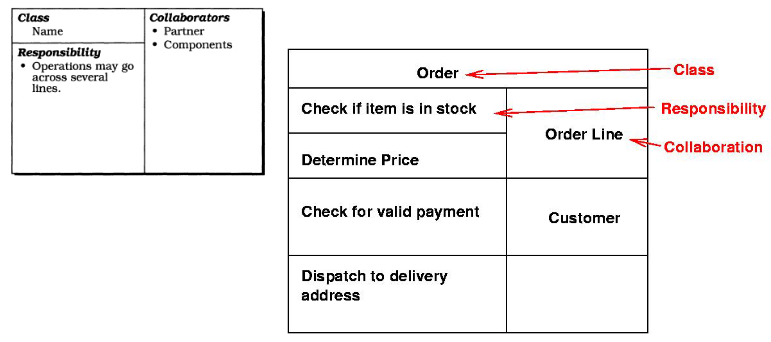
\includegraphics[width=0.5\textwidth]{figures/crc_es.png}
          \end{center}
        \end{figure}
  \section{System Domain Model}
    Nel progetto di dettaglio bisogna passare dalle responsabilità alle operazioni necessarie a realizzare le responsabilità di ciascuna classe: ognuna di queste può essere realizzata attraverso molteplici operazioni. Le operazioni che implementano una responsabilità sono normalmente dichiarate \textit{public}, mentre altri metodi che collaborano a realizzarle devono essere dichiarate, se possibile, \textit{private}. 
    \subsection{Esempio}
      \begin{figure}[h!]
        \begin{center}
          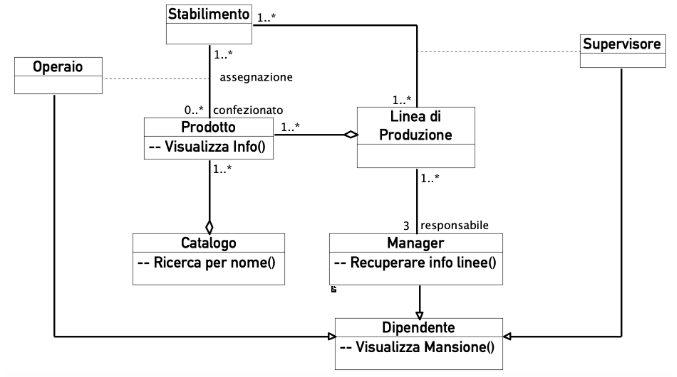
\includegraphics[width=0.5\textwidth]{figures/sdm_es.png}
        \end{center}
      \end{figure}
\end{document}
